%%% Testing:spacing
\documentclass[12pt]{article}


%\usepackage[showboxes]{textpos}

\hoffset=0pt
\voffset=0pt
\oddsidemargin=0pt
\topmargin=0pt
\headheight=0pt
\headsep=0pt

\usepackage{tikz}
\usepackage{graphicx}
\usepackage{esvect}
\usepackage{sistyle}
\usepackage{textpos}

\setlength{\TPHorizModule}{50pt}
\setlength{\TPVertModule}{\TPHorizModule}

% geometry
\usepackage{geometry}
\geometry{ headsep=20pt,
headheight=20pt,
left=21mm,
top=15mm,
right=21mm,
bottom=15mm,
footskip=20pt,
includeheadfoot}

%for using code
\usepackage{listings}
\usepackage{color}

\definecolor{dkgreen}{rgb}{0,0.6,0}
\definecolor{gray}{rgb}{0.5,0.5,0.5}
\definecolor{mauve}{rgb}{0.58,0,0.82}

\lstset{frame=tb,
  language=Java,
  aboveskip=3mm,
  belowskip=3mm,
  showstringspaces=false,
  columns=flexible,
  basicstyle={\small\ttfamily},
  numbers=none,
  numberstyle=\tiny\color{gray},
  keywordstyle=\color{blue},
  commentstyle=\color{dkgreen},
  stringstyle=\color{mauve},
  breaklines=true,
  breakatwhitespace=true,
  tabsize=3
}


% For Multiple Columns within Text
\usepackage{multicol}

% For Links to Websites
\usepackage{hyperref}
\hypersetup{
    colorlinks=true,
    linkcolor=blue,
    filecolor=magenta,      
    urlcolor=cyan,
} 

%plots
\usepackage{pgfplots}

%for the table
\usepackage{multirow}
\usepackage{longtable}
\usepackage{array}
\usepackage{booktabs, tabularx}
\usepackage{caption}
\captionsetup[table]{position=above, belowskip=4pt}
\usepackage{ragged2e}

\usepackage{multicol}
\usepackage{blindtext}

\pagestyle{empty}

%for table with [H]
\usepackage{float}

\title{Dummi}



\begin{document}

	%OnlyPlot
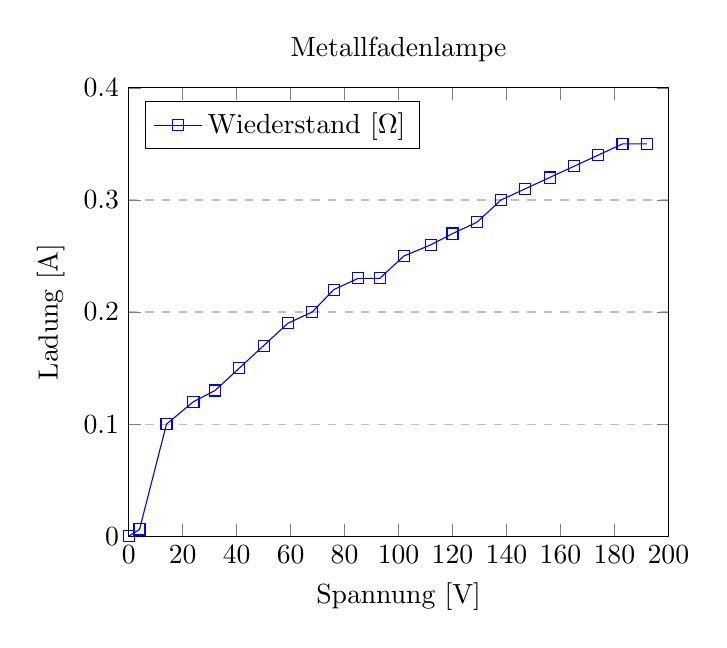
\begin{tikzpicture}
\begin{axis}[
    title={Metallfadenlampe},
    xlabel={Spannung [V]},
    ylabel={Ladung [A]},
    xmin=0, xmax=200,
    ymin=0, ymax=0.4,
    xtick={0,20,40,60,80,100,120,140,160,180,200},
    ytick={0, 0.1, 0.2, 0.3, 0.4},
    legend pos=north west,
    ymajorgrids=true,
    grid style=dashed,
]

\addplot[
    color=blue,
    mark=square,
    ]
    coordinates {
    (0,0)(4,0.006)(14,0.1)(24,0.12)(32,0.13)(41,0.15)(50,0.17)(59,0.19)(68,0.2)(76,0.22)(85,0.23)(93,0.23)(102,0.25)(112,0.26)(120,0.27)(129,0.28)(138,0.3)(147,0.31)(156,0.32)(165,0.33)(174,0.34)(183,0.35)(192,0.35)
    };
    \legend{Wiederstand [$\Omega$]}
    
\end{axis}




\end{tikzpicture}

\begin{center}
    \begin{tabular}{ |  p{8cm}  |   p{8cm}  |}
    \hline  

        Befehl  &   Funktion\\
        \hline
        https://missing.csail.mit.edu/2020/version-control/	& \\
        \hline
        git push ("remote" "local branch":"remote branch")	neue    &    version/veränderungen online speichern \\
        \hline
        git status	    &   status \\
        \hline
        git commit -m "…"	&   neue version local speichern/ takes a snapshot of files and folders and add a message \\
        \hline
        git add	    &   adds files that will be included in next commit \\
        \hline
        git pull	&   meine Version local wird mit der online version überschriben/ same as git fetch; git merge \\
        \hline
        git fetch	&   online version runterladen \\
        \hline
        git init	&   kreate an empty Git repository or reinitialize an existing one \\
        \hline
        git help ...	& \\
        \hline
        git log	    &   shows git history in linear order \\
        \hline
        git log --all --graph --decorate	&   " " but like a graph \\
        \hline
        " " —oneline	 &  " " shorter \\
        \hline
        git checkout "hash/name"	&   brings you to the point of that commit \\
        \hline
    \end{tabular}
\end{center}


    \vfill\noindent
    \begin{tabular}[t]{@{}l} 
        Adresse: \\
        Email: \\
        Mobile: \\
        Geburtsdatum: \\
        Nationalität: \\
        Zivilstand: \\
    \end{tabular}
    \hfill% move it to the right
    \begin{tabular}[t]{l@{}}
        Michelbacherstrasse 6\\
        CH-4055, Basel-Stadt\\
        simon.hammer@gmx.ch \\
        +41 667 73 67 \\
        1. Juli. 2002 \\
        Schweizer \\
        Ledig 
    \end{tabular}

\end{document}
